\section{Results}

\subsection{Seen Object Classes}
First we train an organ-specific CNN on the left atrium data. We choose it as it is the smallest (20 images) since this will be representative of user datasets.

\subsubsection{Training CNN}

\begin{figure}[h!]
\centering
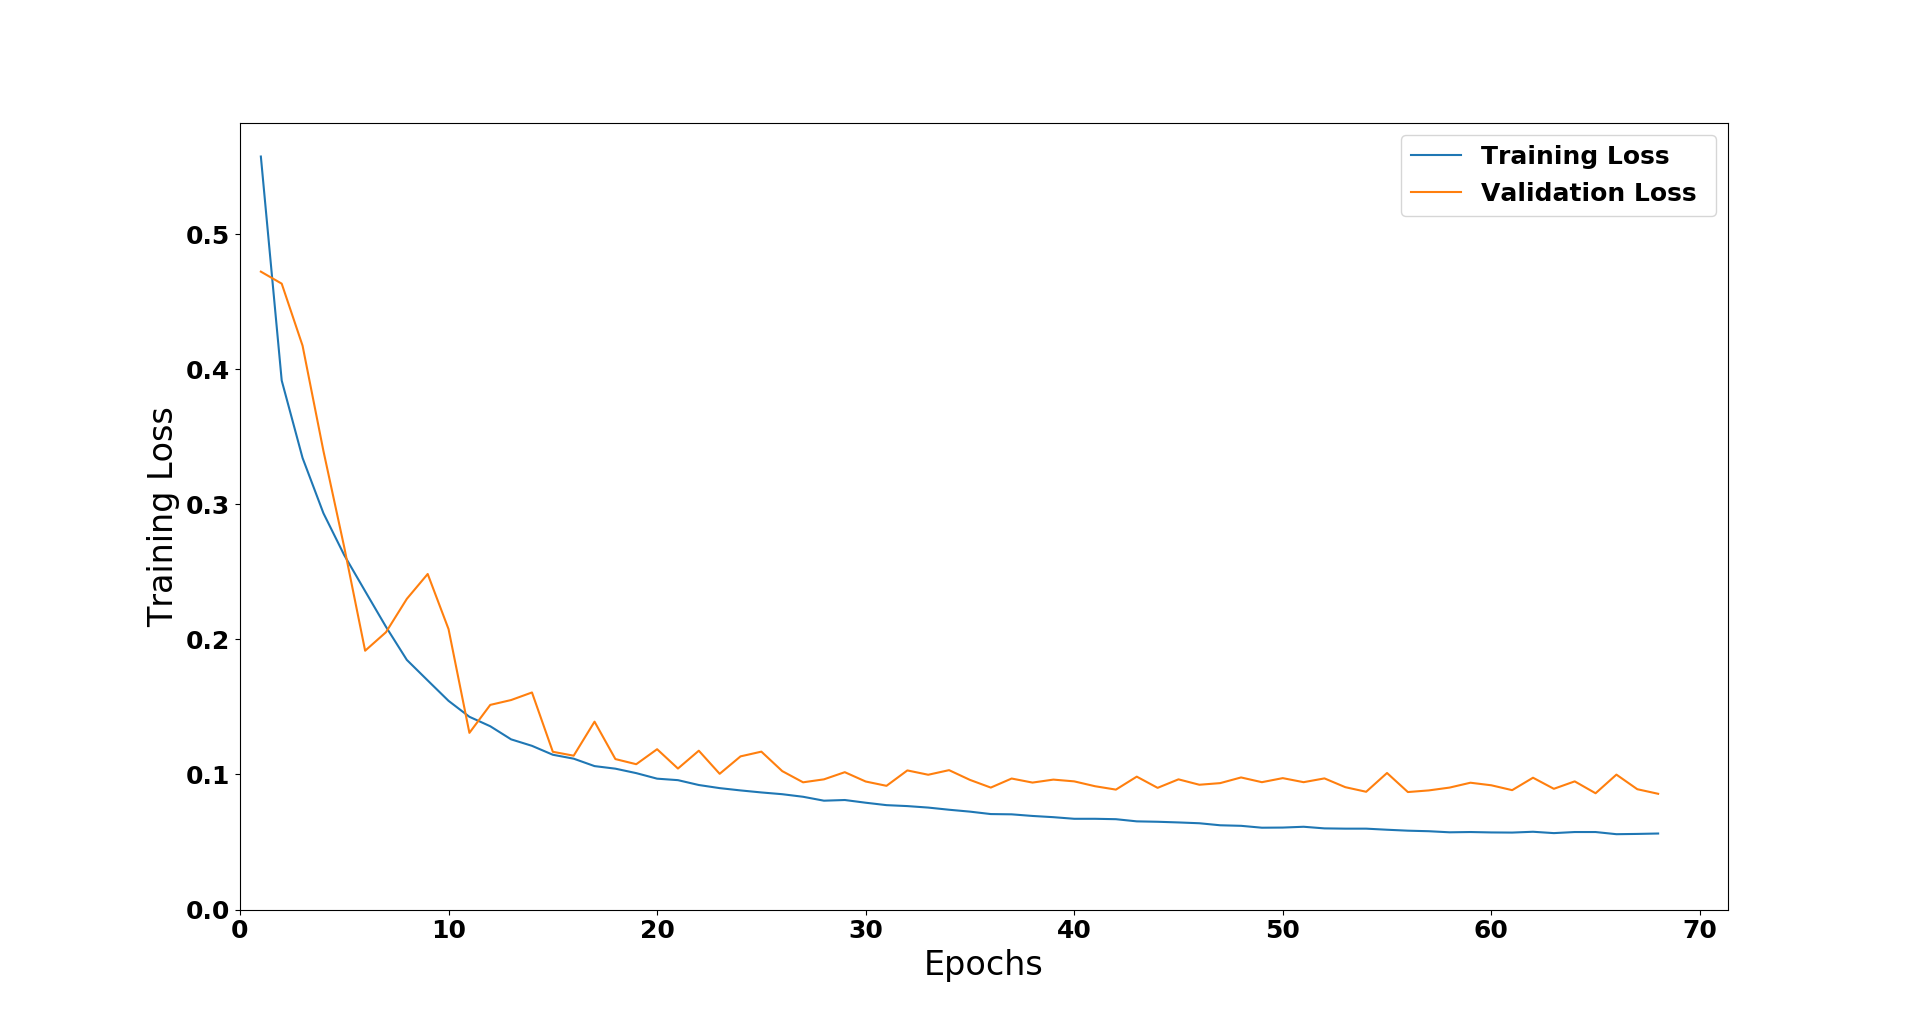
\includegraphics[scale=0.25]{pictures/heartLoss}
\caption{The weighted dice coefficient training and validation loss over time for a dataset of 20 MRI scans and corresponding left atrium segmentations. The training data comprises of 15 images augmented to 90 via random bounding boxes}
\label{fig:lossHeart}
\end{figure}

The dataset is split into 15 training images and 5 validation images. The images are augmented to 90 with different bounding boxes. A learning rate scheduler is used to reduce the learning rate by a factor of 0.5 when no improvement is seen in the validation accuracy after 5 epochs. Learning stops after there has been no improvement in the validation accuracy for 8 epochs. The resulting loss curve is shown in figure \ref{fig:lossHeart}, and the Dice score across the validation set is $0.872 \pm 0.25$.

\subsubsection{Hyperparameters}
This framework has hyperparameters which are not directly related to the CNN, which can be broken up in 2 groups:
\begin{itemize}
\item Those related to the CRF equation, $\lambda$ and $\sigma$ (see Eq. \ref{eq:boundTerm})
\item Those related to the user interactivity (see section \ref{BIFSeg}): $w$, $t_0$, $t_1$, $\sigma_g$, $l$ and those related to fine-tuning, like the number of iterations 
\end{itemize}
The first step is for the CNN to produce a probability map and for this to be used by the CRF to produce a segmentation, without user input. This step depends therefore only on the CRF hyperparameters, so we choose to grid search for these first.

\subsubsection{Graph Cuts Hyperparameters}
A grid search was performed for $\lambda$ and $\sigma$ over the validation set, using the Dice score. As is often done, first a coarse grid search is done and then a finer-grained one, in whichever grid is considered optimal during the coarser search.

\begin{table}[h!]
\centering
\begin{tabular}{|r|r|r|r|}
\hline
               & $\sigma = 0.1$    & $\sigma = 0.5$    & $\sigma=1$        \\ \hline
$\lambda=0.1$  & $0.872 \pm 0.025$ & $0.872 \pm 0.025$ & $0.872 \pm 0.025$ \\ \hline
$\lambda=1$    & $0.875 \pm 0.023$ & $0.876 \pm 0.022$ & $0.873 \pm 0.025$ \\ \hline
$\lambda=10$   & $0.873 \pm 0.025$ & $0.874 \pm 0.024$ & $0.871 \pm 0.025$ \\ \hline
\end{tabular}
\caption{Results for the coarse grid search}
\label{tab:gridCRF}
\end{table}

The results in Table \ref{tab:gridCRF} show that adding a conditional random field results in a marked improvement in the Dice score. Small values of $\lambda$ will make the pairwise terms unimportant relative to the regional terms, while large values of $\sigma$ will make all pairwise terms very similar, thus reducing the relative importance of placing a boundary at places with different intensities. The image is normalised such that it's standard deviation is set to 1, which means $\sigma$ needs to be roughly on that order of magnitude to detect meaningful changes. Too large a value of $\lambda$ hands too much power over to the pairwise potentials, and we see that the Dice scores suffer as a result.

There is inevitably a range of $\lambda$, $\sigma$ for which the Dice scores outperform the case without the CRF (measure by paired t-test at 5\% confidence) but do not outperform each other (20\% confidence). We decide to opt for the largest value of $\lambda$ within this range, on the basis that larger $\lambda$ will be useful for unseen object classes, when the CNN's predictions are likely to be less accurate. The final values chosen are $\lambda=8$, $\sigma=0.2$ which give a Dice score of $0.878 \pm 0.024$.

\subsubsection{BIFSeg Hyperparameters} \label{sec:BIFhyper}
The BIFSeg hyperparameters need user input. We run the CNN over 2 of the validation images and user scribbles are manually added in a broad-stroke manner as in figure \ref{fig:BIFSegEx}. No more than 6 sets of scribbles are added per image in attempt to control for user interaction across images, although ideally performance would be measured with a live user. A grid search for the optimal hyperparameters is then performed, and the average Dice score is the quantity that it optimized for. The other 3 images are then used as a test set for measuring performance. We find that we are able to increase validation Dice scores from the previous value of $0.872 \pm 0.025$ to $0.912 \pm 0.018$, with hyper-parameters $\sigma_g = 0.2$, $l=0$, $t_0=0.6$, $t_1=0.4$, $\epsilon=0.3$, $w=100$, and a learning rate of $2 \cdot 10^{-3}$ for 10 iterations, 10 iterations and then 5 iterations

\subsection{Unseen Object Classes}

\begin{figure}[h!]
\centering
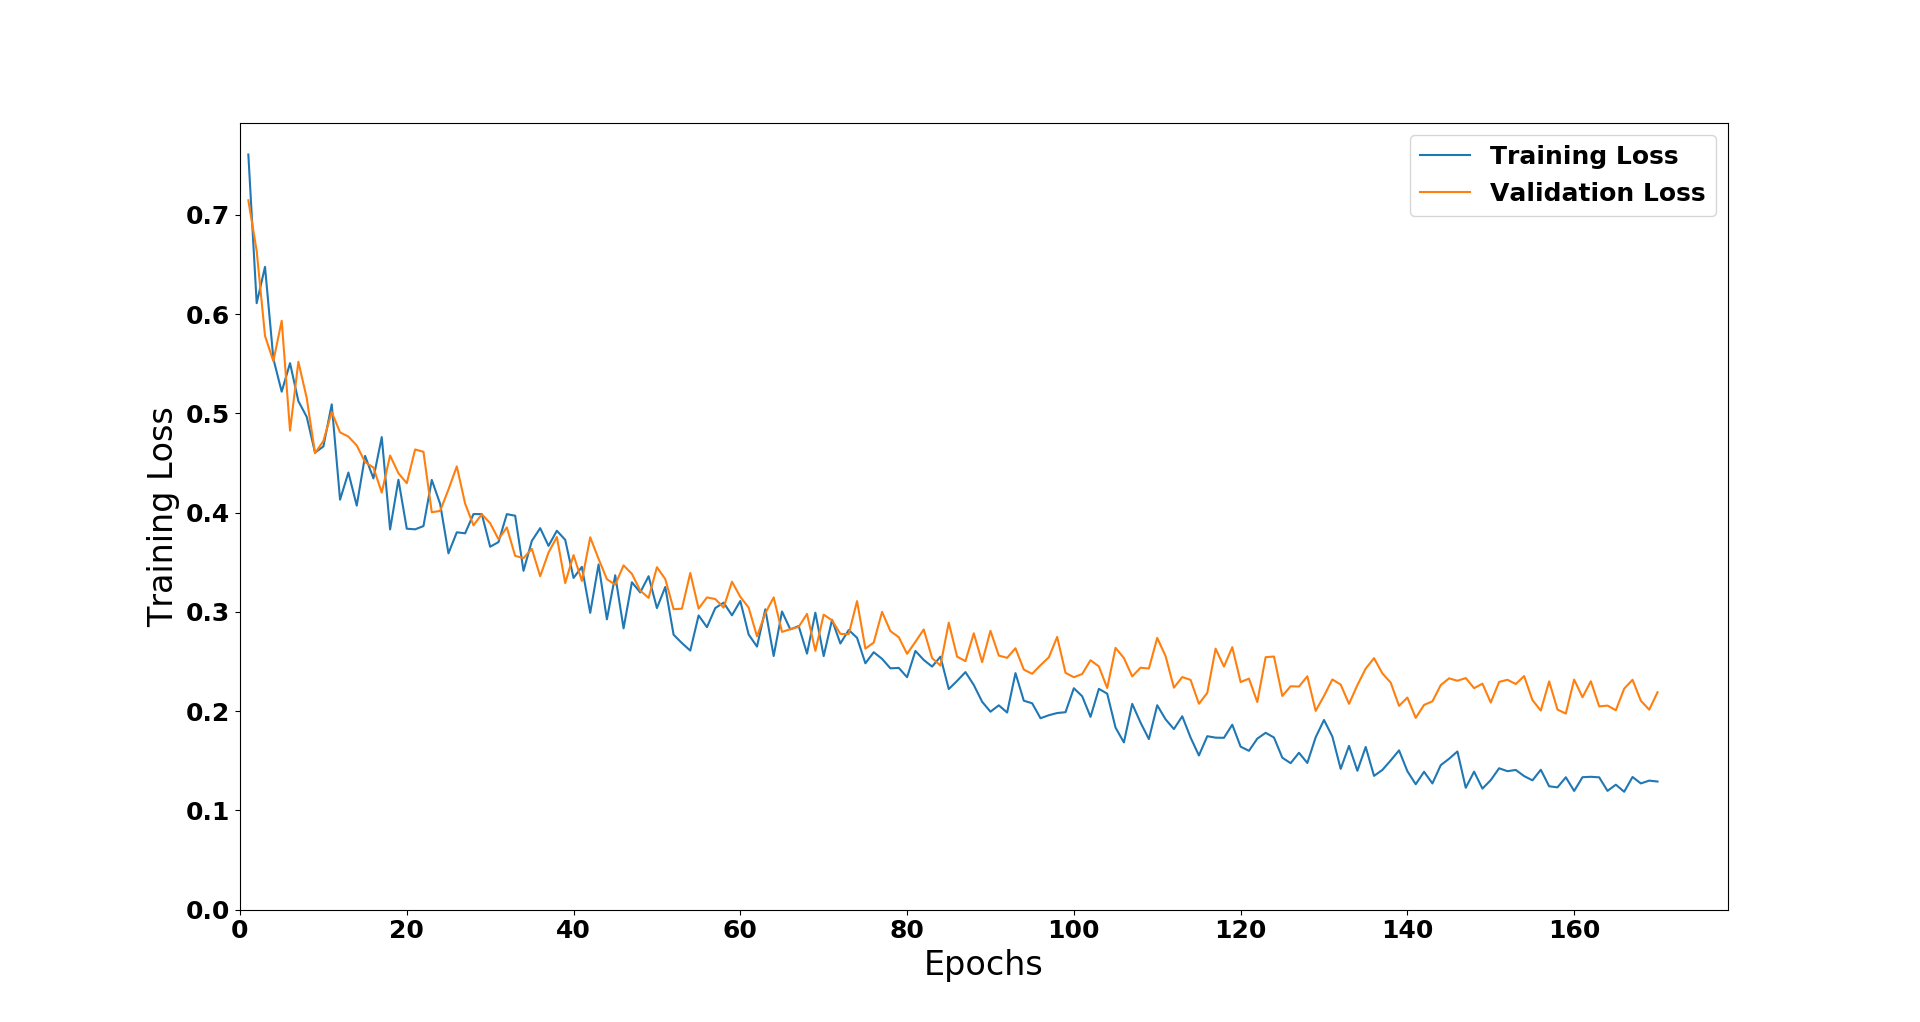
\includegraphics[scale=0.25]{pictures/lossPlotGen}
\caption{The weighted dice coefficient training and validation loss over time for a dataset comprising of 90 training images and 15 validation images split evenly between left atrium, prostate and hippocampus}
\label{fig:lossGen}
\end{figure}

\begin{table}[h!]
\centering
\begin{tabular}{|l|l|}
\hline
Organ Type   & Dice Score         \\ \hline
Left Atrium  & $0.616 \pm 0.025$ \\ 
Prostate     & $0.873 \pm 0.054$ \\ 
Hippocampus  & $0.487 \pm 0.125$ \\ \hline
All          & $0.617 \pm 0.054$ \\ \hline
\end{tabular}
\caption{Validation scores for the generalized segmentation CNN on the organs it was trained on}
\label{tab:resGen}
\end{table}

While the left atrium CNN performs well on the object class it has been trained with, it has not learned any generalisable features - the Dice score over spleen and liver images is $0.093 \pm 0.043$, with some images scoring as low as 0. Even with heavy user interaction, it would be difficult to produce a good segmentation. A new CNN is trained over 3 different organ classes - left atrium, prostate and hippocampus - such that more generalisable features will be learned, rather than features which apply only to one object class. The CNN fails to perform as well on the left atrium as when it was trained on only left atrium images. In fact, in most cases the CNN does perform a segmentation - just a larger one than necessary. The overall validation Dice score is $0.617 \pm 0.054$, and details are shown in table \ref{tab:resGen}. 

\begin{figure}[h!]
\centering
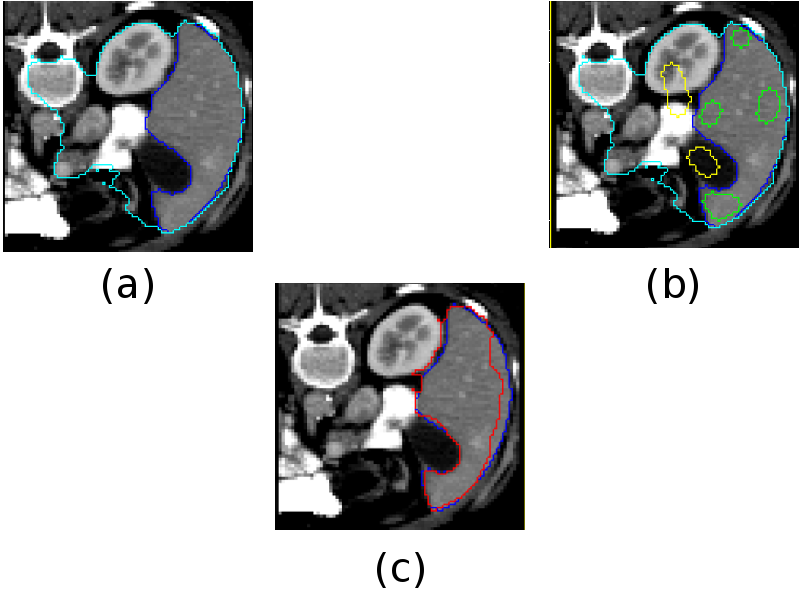
\includegraphics[scale=0.4]{pictures/genBIFSEG.png}
\caption{The process of making and correcting a prediction on a liver, an unseen object type, showing one of the 2D image slices with 6 sets of scribbles. In blue is the ground truth, in cyan the initial guess, in yellow is background scribbles, in green the foreground scribbles and in red is the final segmentation. As expected, the initial segmentation is poor since the CNN does not know what organ it is supposed to be segmenting. The final segmentation  is much improved (0.884 across the whole 3D image) but it has forgotten some information which was previously correct (right hand boundary), and thus adding extra scribbles may boost performance further}
\label{fig:genBIFSeg}
\end{figure}


\begin{table}[h!]
\centering
\begin{tabular}{|l|l|l|}
\hline
Organ Type   & Dice Score (CNN)  & Dice Score (CNN+CRF) \\ \hline
Liver        & $0.516 \pm 0.019$ & $0.532 \pm 0.022$\\ 
Spleen       & $0.417 \pm 0.033$ & $0.484 \pm 0.037$ \\ \hline
\end{tabular}
\caption{Dice scores by the generalized segmentation CNN on unseen object types with and without the CRF}
\label{tab:resGenUnseen}
\end{table}

The validation score on the trained organs is not a particularly interesting or representative measure of performance since this CNN will be used exclusively on object types for which we do not already have a trained CNN (unseen object types). We can look at the Dice score on the spleen and liver organs, which the CNN has never seen (table \ref{tab:resGenUnseen}). As expected they perform worse than on the organs they have seen, but not by much and they still perform significantly better then the CNN trained solely on the left atrium. The high value of $\lambda$ works to boost Dice scores significantly. 

\begin{table}[h!]
\centering
\begin{tabular}{|l|l|l|}
\hline
Organ Type   & Dice Score (10 scribbles) & Dice Score (15 scribbles) \\ \hline
Liver        & $0.873 \pm 0.029$ & $0.891 \pm 0.021$\\ 
Spleen       & $0.892 \pm 0.018$ & $0.918 \pm 0.016$ \\ \hline
\end{tabular}
\caption{Dice scores by the generalized segmentation CNN on unseen object types, after fine-tuning with user interaction}
\label{tab:resGenBIFUnseen}
\end{table}

These Dice scores are obviously still far too low, and this is why we chose to allow for user corrections. As expected, more user interaction is required on unseen objects. We allow for 10 sets of scribbles initially, and the addition of another 5 after a first attempt. The BIFSeg hyperparameters are grid searched over all the validation images, and our test set is the unseen images. We find the same hyperparameters to be optimal as in the case of the left atrium, that is $t_0=0.6$, $t_1=0.4$, $\epsilon=0.3$, $\lambda=8$, $\sigma=0.2$, $w=100$, and a learning rate of $2 \cdot 10^{-3}$ for 10 iterations, 10 iterations and then 5 iterations. Table \ref{tab:resGenBIFUnseen} shows the results. User interaction improves performance significantly, but during the fine-tuning process, the CNN may "forget" things that it previously knew. Seeing the result of the first attempt and adding more scribbles can boost performance significantly in the case of unseen objects, although it takes twice as long.

Figure \ref{fig:genBIFSeg} shows an example of a liver segmentation. The intial segmentation in figure \ref{fig:genBIFSeg}a) is poor if we judge it by it's Dice score, but we can see that the CNN has made a reasonable attempt at segmentation, it just does not know which organ it is meant to be segmenting, and therefore includes anything it can differentiate as an object. 6 of the 10 scribbles are shown in figure \ref{fig:genBIFSeg}b), and \ref{fig:genBIFSeg}c) shows they are enough to provide a much improved segmentation (Dice score 0.884 throughout the 3D volume).   


\subsection{Transfer Learning}

\begin{figure}[h!]
\centering
\makebox[\textwidth][c]{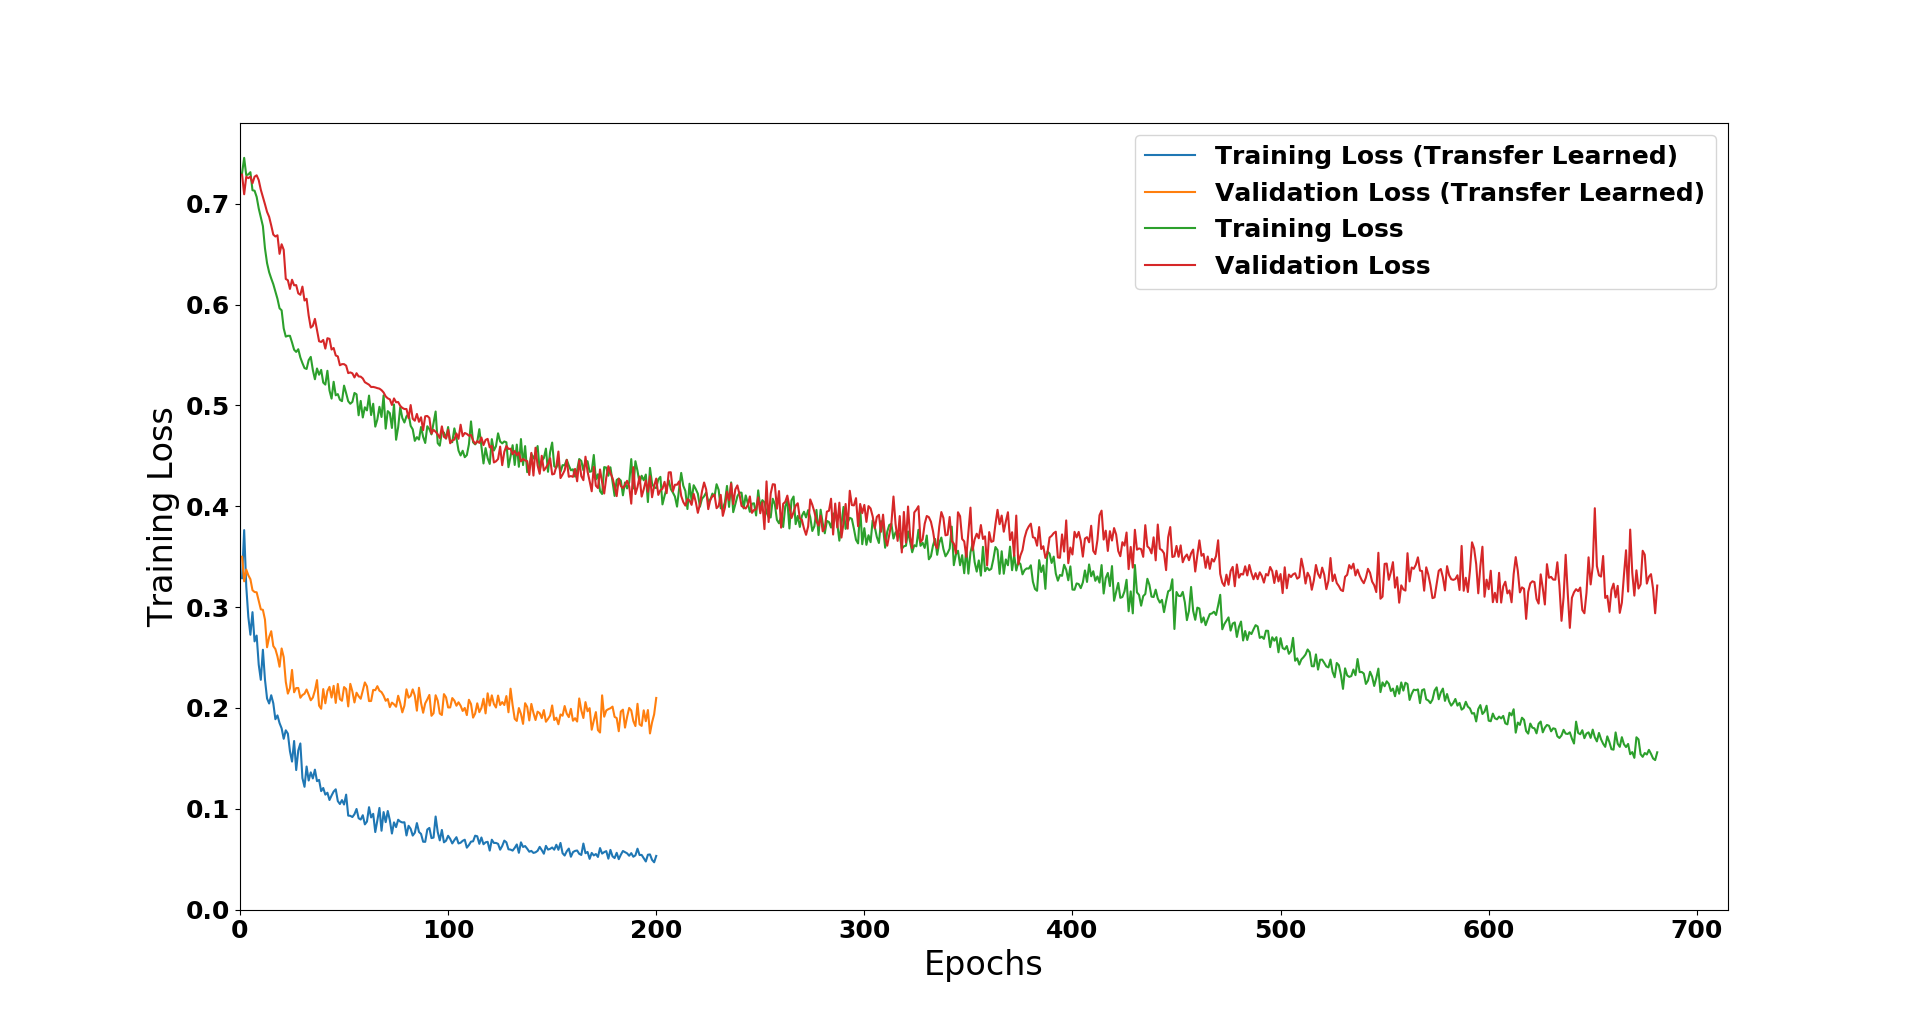
\includegraphics[scale=0.25]{pictures/transferSpleen}}
\caption{The loss curves of the CNN training on 4 spleen images and validating on 6, in one case it is pre-loaded with weights from a generalised CNN, in the other it is trained from scratch. The small datasets mean that both end up heavily overfitting, but the performance and learning speed of the transfer learned CNN is still far surperior.}
\label{fig:lossTransSpleen}
\end{figure}

\begin{figure}[h!]
\centering
\makebox[\textwidth][c]{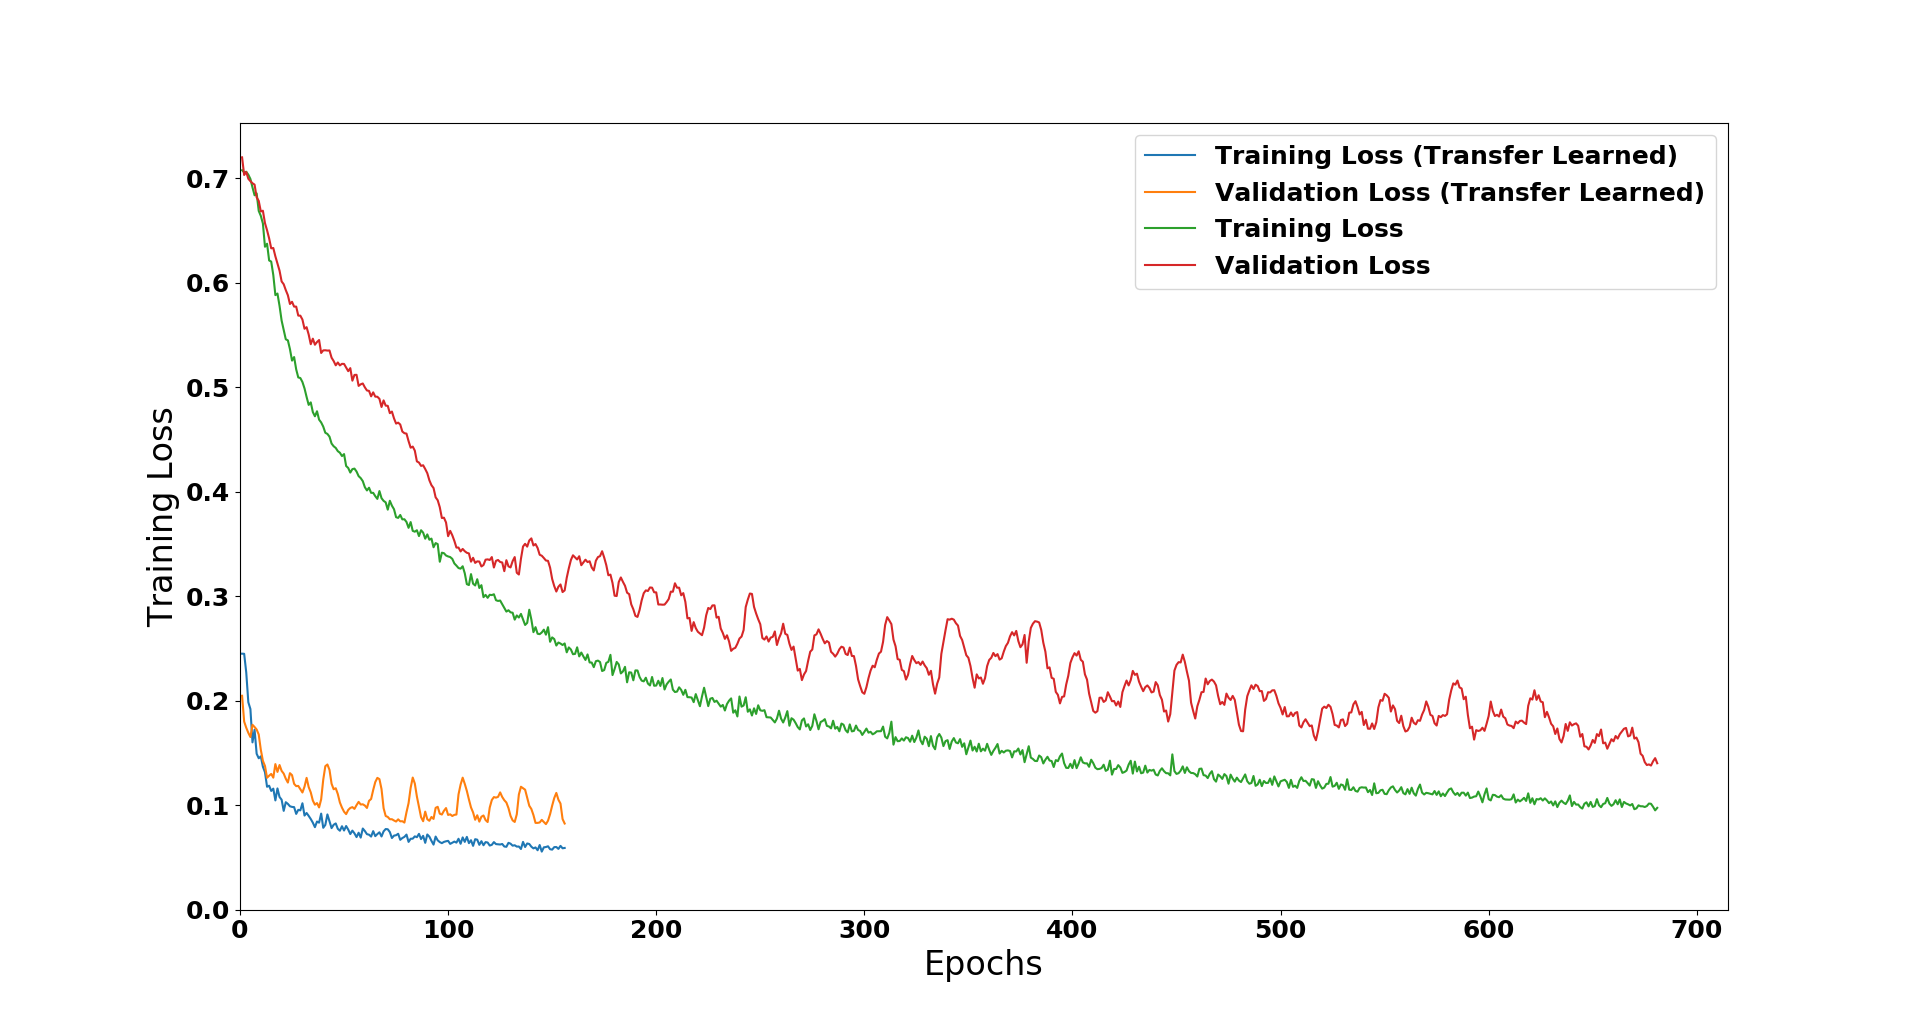
\includegraphics[scale=0.25]{pictures/transferLiver}}
\caption{The loss curves of the CNN training on 4 liver images and validating on 6, in one case it is pre-loaded with weights from a generalised CNN, in the other it is trained from scratch. The small datasets mean that both end up overfitting, but the performance and learning speed of the transfer learned CNN is still far surperior.}
\label{fig:lossTransLiver}
\end{figure}


In order to test the efficacy of transfer learning in this framework, a small training dataset of 4 training images and 6 validation images is produced. This is intended to simulate what a user might submit, after having made a few successful segmentations with the generalized segmentation CNN. First the CNN is trained from scratch on these images. Then, a new CNN is created and the weights from the generalised segmentation CNN are transferred to that of the new CNN. This CNN is then trained on the same dataset. Note that this is not fine-tuning: both sides of the U shape are trained in this case. A constant learning rate of $2 \cdot 10^{-4}$ is used in both cases so that speed and quality of convergence may be compared on a roughly equal footing, adn we stop agter no improvement has been seen in 10 epochs. Since we are training on such a small dataset, we do not expect state of the art performance on the validation set, but we still aim for a significant improvement over the unseen case. Figure \ref{fig:lossTransSpleen} shows the loss curves for the spleen. Both CNNs produce heavy overfitting, as would be expected from such a small dataset. However, the transfer learned CNN performs better and faster. It produces a best case validation loss of 0.19 by epoch 100, whereas it takes four times as long for the CNN learning from scratch to reach a validation loss which is still over twice as high (0.41). The best case validation loss for the transfer learned CNN is 0.18 and for the CNN learning from scratch, 0.34. The ratios are similar for the liver (figure \ref{fig:lossTransLiver}), although overfitting is less significant.

This confirms, at least for the cases of the liver and the spleen, that the information learned in the original training was generalizable enough to minimize overfitting on a small dataset, improve performance and improve training speed. From this data, a CNN can be trained to perform adequately within 50-100 epochs with transfer learning and 500-1000 epochs without it - an order of magnitude improvement. For 4 images with a rather large but not uncommon bounding box size of 128x128x128, this changes the total training time from being on the order 15-30 hours to being on the order of 1.5-3 hours.

\subsection{Timings}
Evaluating the value of this framework would entail timed tests with medical staff using this framework and other frameworks, in order to compare accuracy and speed. Wang et al. did perform some limited tests in which BIFSeg performed at least as accurately as existing methods. It's main advantage was that it required much less user interaction than the other frameworks, and therefore performed faster in terms of total user time. Unfortunately, at the time of writing, no such tests have been performed for this framework. 

There is one clear source of added time, that is network latency - when the images and segmentations are sent to and from the server. Large images can easily take up several megabytes, and this transfer can take on the order of several seconds depending on the quality of the network connection. However, this is generally 10\% or less of the total time, with the the only other signficant source of machine time being the fine-tuning process.

Since the network is a fully convolutional network, it takes images of any size, and we do not do any rescaling. The CRF also works on images of any size. As a result, the time taken can vary wildly depending on the size of the image. Ignoring network latency, a single inference on a 32x32x32 image will take a fraction of a second, whereas an 80x80x80 (15 times as many pixels) will take on the order of 2-3 seconds. 

